%% abtex2-modelo-trabalho-academico.tex, v<VERSION> laurocesar
%% Copyright 2012-<COPYRIGHT_YEAR> by abnTeX2 group at http://www.abntex.net.br/ 

\documentclass[
	% -- opções da classe memoir --
	12pt,				% tamanho da fonte
	oneside,			% para impressão mudar para twoside para facilitar impressaõ de frente e verso 
	a4paper,			% tamanho do papel. 
	chapter=TITLE,
	sumario=tradicional,
	% -- opções do pacote babel --
	english,			% idioma adicional para hifenização
	brazil				% o último idioma é o principal do documento
]{abntex2}

% ----------------------------------------------------------
% IMPORTAÇÃO DE PACOTES
% ----------------------------------------------------------
\usepackage{helvet}
\renewcommand{\familydefault}{\sfdefault}			% Usa a fonte Arial			
\usepackage[T1]{fontenc}		% Selecao de codigos de fonte.
\usepackage[utf8]{inputenc}		% Codificacao do documento (conversão automática dos acentos)
\usepackage{indentfirst}		% Indenta o primeiro parágrafo de cada seção.
\usepackage{color}				% Controle das cores
\usepackage{graphicx}			% Inclusão de gráficos
\usepackage{microtype} 			% para melhorias de justificação
\usepackage{hyperref}
\usepackage{times}
\usepackage{siunitx}

\usepackage{amsmath}
\usepackage{amsthm,amsfonts}

\usepackage{lipsum}				% para geração de dummy text
\usepackage{import}
\usepackage{blindtext}
\usepackage{soul}
\usepackage{lscape}
\usepackage{float}

\graphicspath{ {./images/} }

% ---
% Pacotes de citações
% ---
\usepackage[alf]{abntex2cite}	% Citações padrão ABNT

% ----------------------------------------------------------
% CONFIGURAÇÕES DO PDF
% ----------------------------------------------------------

% alterando o aspecto da cor azul
\definecolor{blue}{RGB}{41,5,195}
\definecolor{black}{RGB}{0,0,0}

% informações do PDF
\makeatletter
\hypersetup{
     	%pagebackref=true,
		pdftitle={\@title}, 
		pdfauthor={\@author},
    	pdfsubject={\imprimirpreambulo},
	    pdfcreator={LaTeX with abnTeX2},
		pdfkeywords={abnt}{latex}{abntex}{abntex2}{trabalho acadêmico}, 
		colorlinks=true,       		% false: boxed links; true: colored links
    	linkcolor=black,          	% color of internal links
    	citecolor=black,        		% color of links to bibliography
    	filecolor=black,      		% color of file links
		urlcolor=black,
		bookmarksdepth=4
}
\makeatother

\setlrmarginsandblock{3cm}{2cm}{*}
\setulmarginsandblock{3cm}{2cm}{*}
\checkandfixthelayout

% --- 

% ----------------------------------------------------------
% FIGURAS E TABELAS
% ----------------------------------------------------------

% ---
% Posiciona figuras e tabelas no topo da página quando adicionadas sozinhas
% em um página em branco. Ver https://github.com/abntex/abntex2/issues/170
\makeatletter
\setlength{\@fptop}{5pt} % Set distance from top of page to first float
\makeatother
% ---

% ----------------------------------------------------------
% ESPAÇAMENTOS
% ----------------------------------------------------------

% O tamanho do parágrafo é dado por:
\setlength{\parindent}{1.25cm}

% % Controle do espaçamento entre um parágrafo e outro:
\setlength{\parskip}{0.2cm} 

\setlength{\ABNTEXcitacaorecuo}{4cm}

% Espaçamento entre headers e texto abaixo
\setlength\afterchapskip{0.2cm}
\setlength\aftersecskip{0.2cm} %espaçamento entre seção e texto
\setlength\aftersubsecskip{0.2cm} %espaçamento entre subseção e texto

% ----------------------------------------------------------
% CORREÇÕES DE ESTILO
% ----------------------------------------------------------

% Estilos das legendos
\captionnamefont{\ABNTEXfontereduzida}
\captiontitlefont{\ABNTEXfontereduzida}
\setlength{\belowcaptionskip}{1pt} % espaçamento depois do título das tabelas/figuras
\setlength{\abovecaptionskip}{1pt} % espaçamento antes da legenda de tabelas/figuras

% Estilos dos títulos

\renewcommand{\ABNTEXchapterfontsize}{\bfseries\normalsize}
\renewcommand{\ABNTEXsectionfontsize}{\itshape\normalsize}
\renewcommand{\ABNTEXsubsectionfontsize}{\normalfont\normalsize}
\renewcommand{\ABNTEXsubsubsectionfontsize}{\normalfont\normalsize}

\renewcommand{\chaptitlefont}{\normalfont\bfseries}
\setsecheadstyle{\normalfont\itshape}
\setsubsecheadstyle{\normalfont}
\setsubsubsecheadstyle{\normalfont}

\renewcommand{\ABNTEXchapterfont}{\bfseries}
\renewcommand{\ABNTEXchapterfontsize}{\normalsize}
\setboolean{ABNTEXupperchapter}{true}

% Estilos nos sumários
\renewcommand{\cftchapterfont}{\MakeUppercase}
\setboolean{ABNTEXupperchapter}{true}

\renewcommand{\cftsectionfont}{\normalfont}
\renewcommand{\cftsubsectionfont}{\normalfont}
\renewcommand{\cftsubsubsectionfont}{\normalfont}

% ----------------------------------------------------------
% COMPILA O ÍNDICE
% ----------------------------------------------------------
\makeindex

% ----------------------------------------------------------
% COMANDOS CUSTOMIZADOS
% ----------------------------------------------------------
\newcommand{\un}[1]{\;\text{#1}}
\newcommand{\logo}{\quad \Rightarrow \quad}
\newcommand{\codeword}[1]{\texttt{\textcolor{black}{#1}}}
\newcommand{\specialcell}[2][c]{%
  \begin{tabular}[#1]{@{}c@{}}#2\end{tabular}}

% ----------------------------------------------------------
% INÍCIO DO DOCUMENTO
% ----------------------------------------------------------
\begin{document}

%\selectlanguage{english}
\selectlanguage{brazil}

% Retira espaço extra obsoleto entre as frases.
\frenchspacing 

% ----------------------------------------------------------
% ELEMENTOS PRÉ-TEXTUAIS
% ----------------------------------------------------------
\begin{center}
\textbf{UNIVERSIDADE FEDERAL DE MINAS GERAIS\\
Escola de Engenharia \\
Curso de Bacharelado em Engenharia de Sistemas}

\vspace{4cm}

%\hspace{0.3\textwidth} \parbox{0.65\textwidth}
Cleyton Luan Nobre Assis 2021019815 \\
Maria Clara Oliveira Domingos Ruas 2021019572 \\
Raphael Henrique Braga Leivas 2020028101

\vspace{4cm}  

{ \textbf{Laboratório de Circuitos Eletrônicos e Projetos - \\ Relatório Fonte de Alimentação} }

\vfill
%\hspace{0.3\textwidth} 
{Belo Horizonte \\
2025 }
\end{center}

\newpage

% ---
% inserir o sumario
% ---
\pdfbookmark[0]{\contentsname}{toc}
\tableofcontents*
\cleardoublepage
% ---

% % ----------------------------------------------------------
% % ELEMENTOS TEXTUAIS
% % ----------------------------------------------------------
\textual

\pagestyle{simple}

\chapter{Introdução}\label{cap:introdução} 

Este relatório é referente ao projeto da fonte de alimentação desenvolvido na matéria de Laboratório de Circuitos Eletrônicos e Projetos em 01/2025. O projeto envolve desde os estudos das partes e funcionamento dos componentes utilizados, escolha e compra dos componentes, simulações do circuito, montagem da placa e testes finais.

A fonte de alimentação é um dispositivo elétrico de extrema importância, capaz de fornecer energia elétrica de forma controlada e estável. Assim, ela consegue alimentar cargas e circuitos, protegendo e garantindo todo o bom funcionamento de aplicações elétricas. O desenvolvimento do projeto é importante para compreender de forma mais aprofundada o funcionamento dos dispositivos e as etapas necessárias para converter a corrente alternada da rede elétrica para corrente contínua, métodos para diminuir a perda energética ainda mantendo uma estabilidade no sinal e proteger a carga de forma eficaz, evitando perdas maiores. 

Além disso, o projeto proporciona uma experiência prática essencial, permitindo a aplicação dos conhecimentos teóricos adquiridos ao longo do curso em situações reais de projeto e montagem. Ao longo do desenvolvimento, foram abordados conceitos como retificação, filtragem, regulação de tensão e dissipação de calor, bem como aspectos relacionados à segurança elétrica e eficiência energética. Dessa forma, este relatório tem como objetivo documentar todas as etapas do processo, desde o planejamento inicial até a análise dos resultados obtidos, destacando os desafios enfrentados, as soluções adotadas e os aprendizados adquiridos.

Todos os componentes e etapas do projeto estão especificados no Capítulo \ref{cap:objetivos}, seguido pela análise em alto nível do funcionamento geral do circuito da fonte dividido em blocos por funcionalidade no Capítulo \ref{cap:estudo_geral}. Após o estudo em alto nível, os cálculos para os componentes são realizados no Capítulo \ref{cap:calculo} e a simulação do circuito no Capítulo \ref{cap:simulacao}.

Seguindo para a parte prática, no Capítulo \ref{cap:resultados}, é apresentado os resultados dos testes e experimentos feitos na placa e a lista dos componentes utilizados para a montagem no Capítulo \ref{cap:lista_componentes}. É feita a análise e discussão dos resultados encontrados no Capítulo \ref{cap:analise} e sugestões para trabalhos futuros no Capítulo \ref{cap:surgestao}. Por fim, o relatório é finalizado com a conclusão do trabalho desenvolvido no Capítulo \ref{cap:conclusao}.


\chapter{Descrição do Projeto}\label{cap:objetivos} 

O projeto apresentado é uma fonte de alimentação simétrica regulada, com saídas positivas e negativas, que permite o controle e monitoramento da tensão e corrente de saída. É composto por uma série de blocos que incluem retificação, geração de tensões auxiliares, referência de tensão, amplificação e proteção, tanto para a parte positiva quanto para a negativa do circuito.

A fonte é projetada para converter uma entrada de corrente alternada (AC) em saídas contínuas (CC) estáveis, protegidas e ajustáveis, adequadas para alimentar dispositivos eletrônicos sensíveis. A presença de circuitos de proteção e controle garante maior segurança e confiabilidade para os equipamentos alimentados.

Na Figura \ref{fig:esquematico}, é possível visualizar todas as partes do projeto a ser desenvolvido, bem como seus pontos de coleta de valores para teste. A função, funcionamento e discussão sobre cada bloco será mais detalhada na próxima sessão.


\begin{figure}[H]
    \centering
    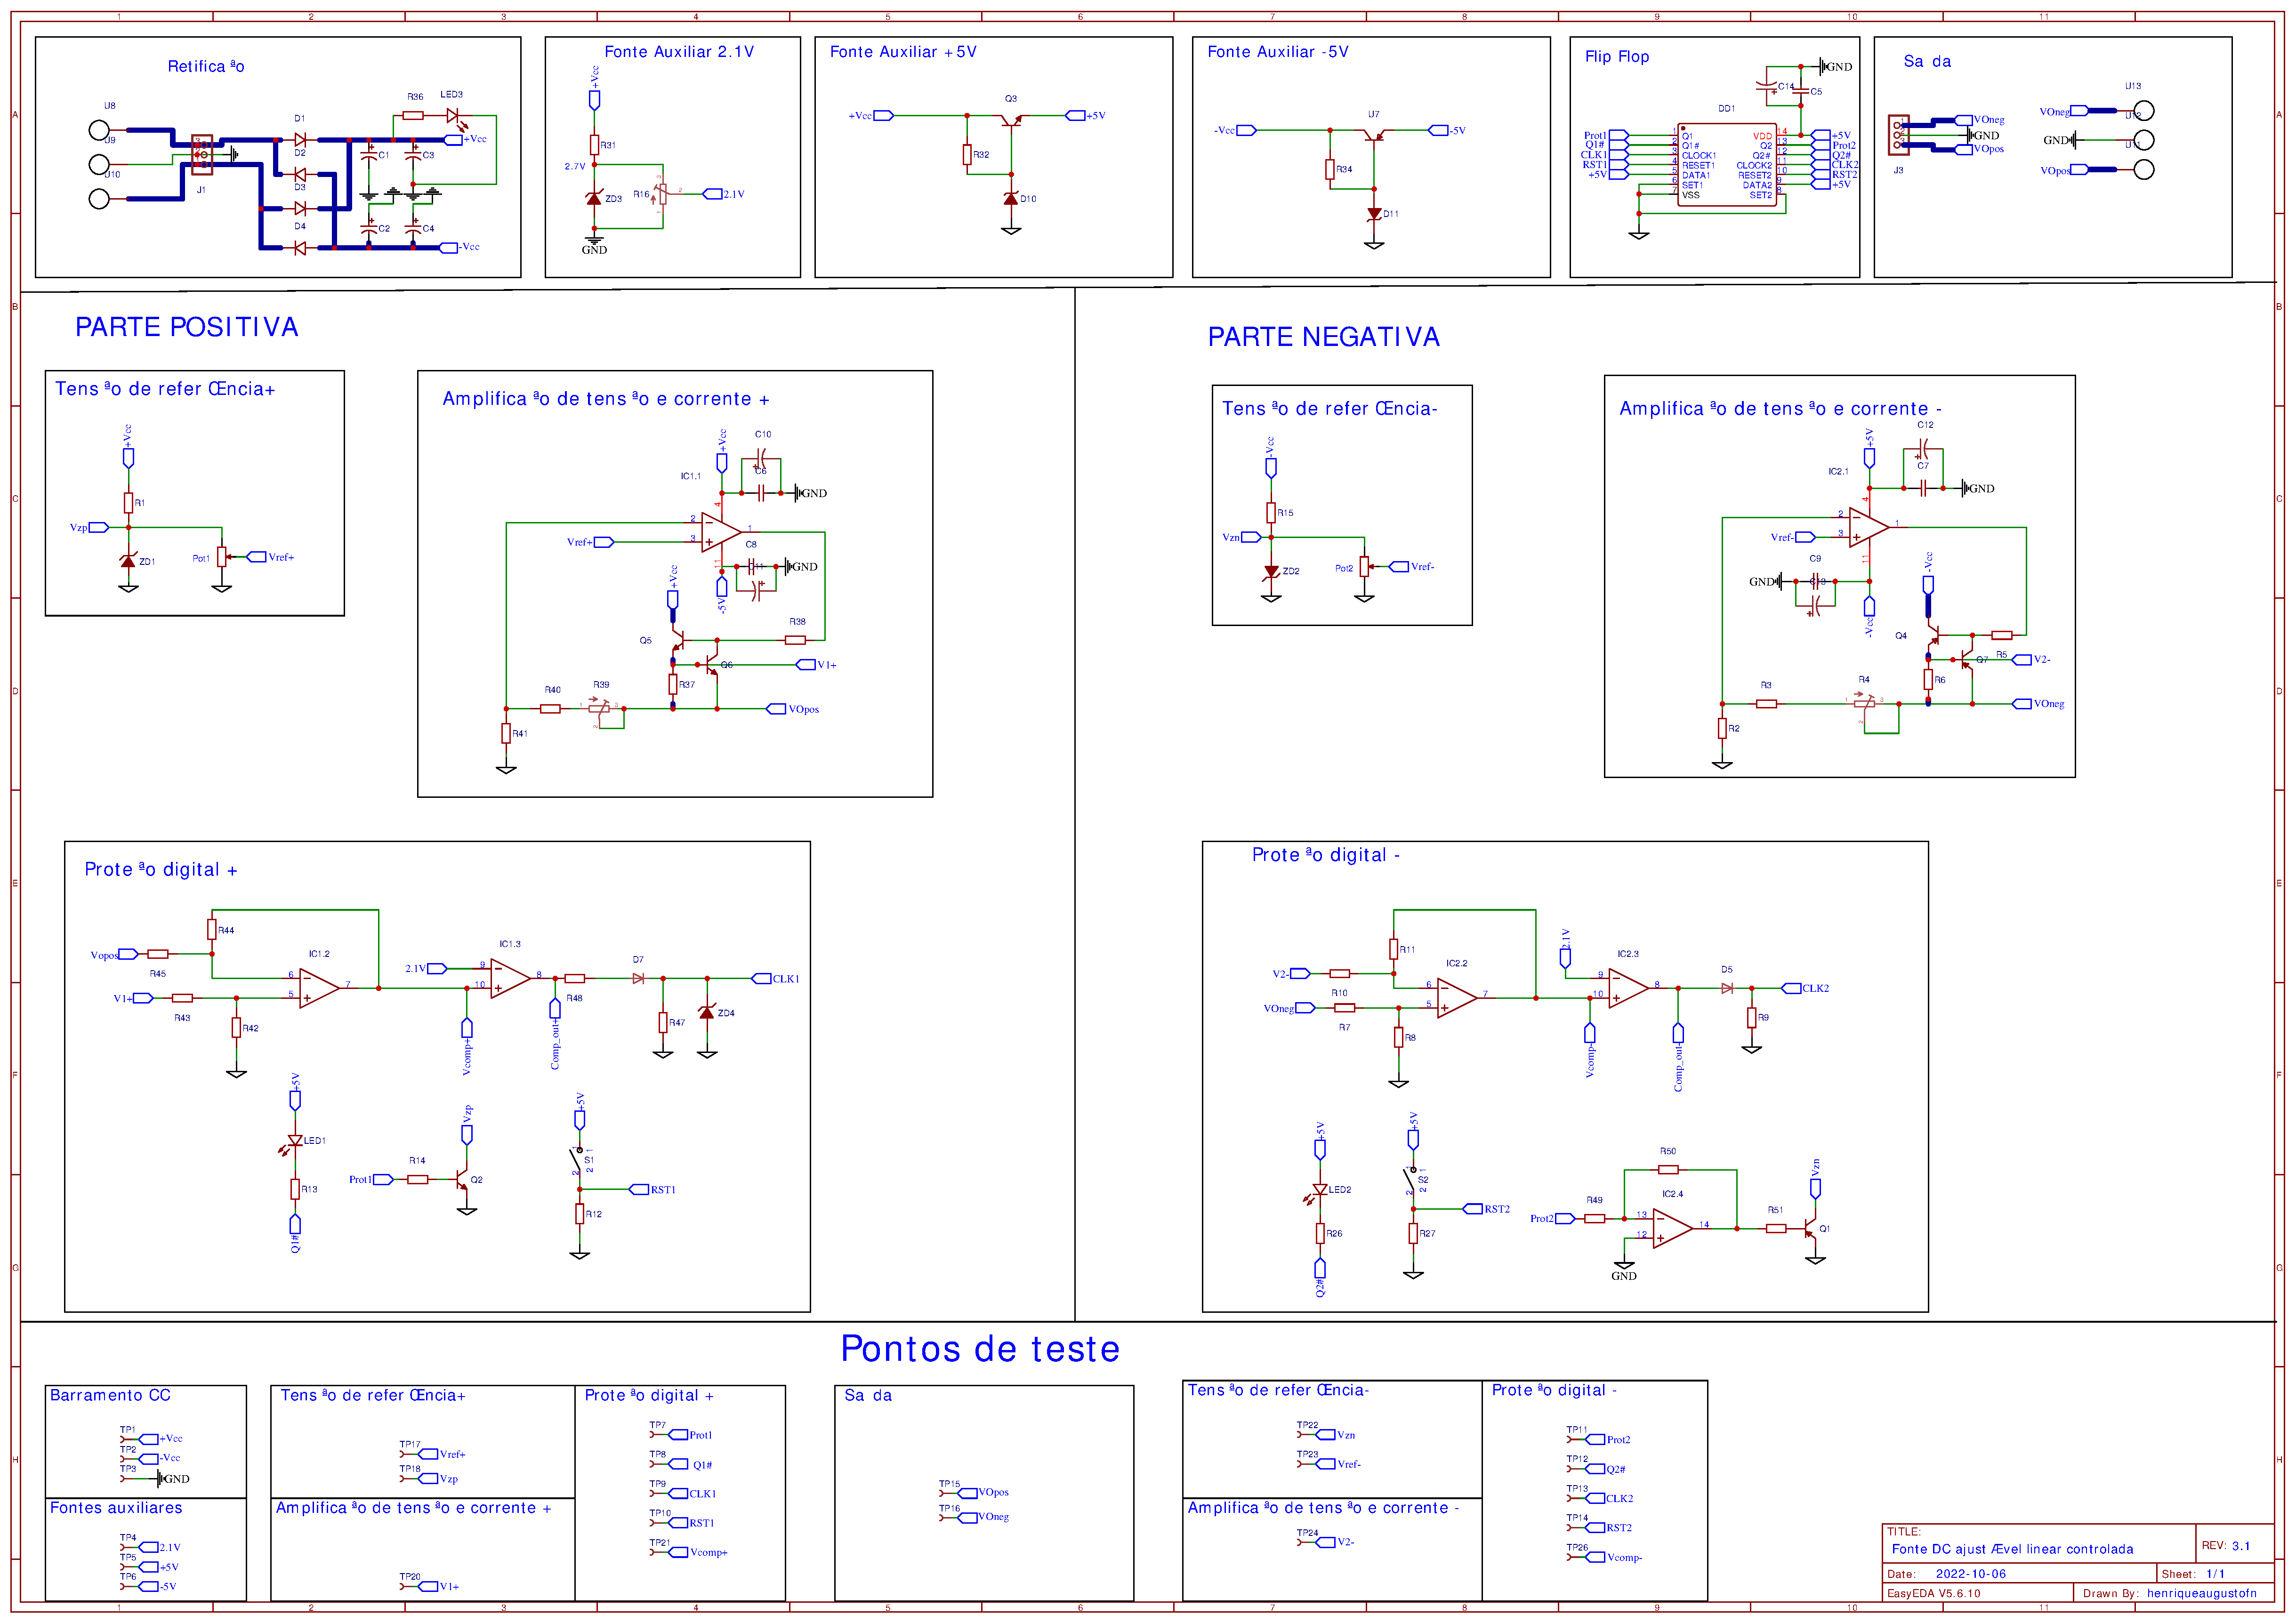
\includegraphics[width=\linewidth]{images/Esquematico.pdf}
    \caption{Esquemático do projeto da fonte sem valores}
    \label{fig:esquematico}
\end{figure}


\chapter{Estudo geral do funcionamento do circuito da fonte dividido em blocos}\label{cap:estudo_geral} 

O primeiro bloco, ``Retificação'', é responsável por converter a tensão alternada , proveniente da rede elétrica ou de um transformador, em uma tensão contínua pulsante. Esse processo é realizado por uma ponte retificadora com quatro diodos, seguida por um capacitor de filtragem que suaviza a tensão de saída. Essa etapa fornece a base de energia contínua sobre a qual os demais circuitos operam. Mesmo com a ação do capacitor, a variação de tensão após está etapa ainda é considerável.

O próximo bloco que foi montado foram os blocos das ``Fontes Auxiliares'', responsáveis por gerar tensões fixas adicionais necessárias para o funcionamento dos circuitos de controle. São elas: +2,1V, +5V e –5V. A fonte de +2,1V é utilizada como referência para os comparadores de proteção digital, enquanto as fontes de \(\pm5V\) alimentam circuitos lógicos e operacionais. Estes blocos utilizam transistores e reguladores lineares para fornecer essas tensões de forma estável, contribuindo diretamente para a precisão e segurança do sistema.

O bloco de ``Flip-Flop'' implementa uma lógica de travamento digital. Esse circuito é utilizado para manter o estado da fonte após uma condição de falha ser detectada, como sobrecorrente ou sobretensão. Uma vez que uma dessas falhas ocorra, o flip-flop pode ser setado e manter o circuito desligado até que seja manualmente resetado, garantindo proteção contínua da carga.

O bloco de ``Saída'' fornece os terminais onde a carga será conectada. Estão disponíveis as tensões de saída positiva (Vout+), negativa (Vout–) e o terra (GND). É a interface final do circuito com o usuário, e qualquer instabilidade ou falha no fornecimento de energia neste ponto pode comprometer o funcionamento dos dispositivos alimentados.

O circuito é dividido internamente em duas grandes seções: parte positiva e parte negativa, que operam de forma espelhada.

Na parte positiva, o primeiro bloco é o de ``Tensão de Referência +'', que utiliza um diodo zener polarizado por um resistor para gerar uma tensão fixa. Essa tensão é usada como base para os comparadores da etapa de controle de tensão e corrente, garantindo estabilidade no ponto de referência.

O bloco seguinte é o de ``Amplificação da Tensão e Corrente +'', que utiliza amplificadores operacionais e transistores de potência para ajustar a tensão de saída com base na referência e nos sinais de feedback. A tensão de saída é constantemente monitorada e comparada com a referência, e o circuito amplifica a diferença para controlar o transistor série, mantendo a saída regulada mesmo com variações de carga.

O bloco de ``Proteção Digital +'' monitora a tensão e corrente de saída e compara esses valores com limites predefinidos utilizando comparadores operacionais. Quando detectada uma condição de falha como sobrecorrente, o circuito envia um sinal para o flip-flop, que desliga a fonte para proteger a carga. Essa proteção é reforçada com o uso de LEDs indicadores, diodos de clamp e transistores de chaveamento.

A parte negativa possui uma estrutura e funcionamento análogos à parte positiva. O bloco de ``Tensão de Referência –'' também usa um zener para gerar uma referência fixa, enquanto o bloco de ``Amplificação da Tensão e Corrente –'' opera com amplificadores e transistores para manter a saída negativa estável. O controle é feito de forma similar, com feedback contínuo da saída para os comparadores.

Por fim, o bloco de ``Proteção Digital'' – realiza as mesmas funções que o seu equivalente positivo, detectando falhas na linha negativa e agindo rapidamente para evitar danos ao circuito ou à carga.



\chapter{Cálculos dos componentes de cada um dos blocos de funcionamento do circuito}\label{cap:calculo} 

Durante o desenvolvimento do projeto da fonte de alimentação simétrica, foram realizados cálculos e escolhas criteriosas dos componentes utilizados em cada bloco funcional, considerando a corrente, tensão, potência e a função de cada elemento no circuito.

\section{Retificador e Filtro Capacitivo}
A etapa de retificação utiliza quatro diodos 1N4007, formando uma ponte retificadora. A corrente média de condução por diodo foi estimada em ao menos 1A, com uma tensão reversa máxima superior ao dobro da tensão de pico da rede transformada:

$$V_{DMax} \geq 2V_{pico}=2.2,45V = 50,8V$$

Como os diodos 1N4007 suportam até 1 A e 1000 V, são adequados para a aplicação.

O filtro capacitivo é responsável por suavizar a tensão contínua após a retificação. A tensão máxima de operação dos capacitores deve ser superior à tensão contínua gerada:

$$V_{CMax} > V_{CC} = 24,7V \implies V_{C nom} = 35V$$

Foram levantadas as configurações com:

$$C_{total} = 3,3mF$$ ou $$C_{1} = 1mF,\ C_2=2,2mF$$

\section{Fonte Auxiliar para Amplificadores Operacionais}

Para alimentar os amplificadores operacionais, foi projetada uma fonte auxiliar baseada em diodos zener de 5,7V ou 6,2V (1N4734 ou 1N4735). O resistor em série com o zener foi calculado com base na corrente mínima de zener e sua potência:

$$I_Z = \frac{V_{CC} - V_Z}{R} < I_{ZMax} \implies 117,9\Omega$$

$$P_R = \frac{(V_{CC} - V_Z)^2}{R} < P_{MaxResistor} = \frac{1}{4}W \implies 1,4k\Omega$$

Foi adotado um resistor de \(2k\Omega\), valor seguro acima do mínimo necessário (\(1,4k\Omega\)), garantindo funcionamento confiável sem sobrecarregar o zener.

\section{Referência de Tensão}

Cada lado da fonte (positivo e negativo) possui um circuito de tensão de referência, usando também zener de 5,1V (1N4734 ou 1N4735), com resistores de \(2,2k\Omega\). Um trimpot de \(10k\Omega\) é adicionado para ajuste fino da tensão de saída.

A condição de valor mínimo para o trimpot é dada por:

$$R_{pot} > \frac{V_Z.R}{V_{CC} - V_Z} = \frac{5,1.2,2k\Omega}{24,7-5,1} \approx 572\Omega$$

Logo, \(10K\Omega\) é uma escolha adequada e segura.

\section{Controle de Corrente}

A referência de corrente utiliza zener de 3,3V, polarizado por resistor para garantir funcionamento dentro dos limites de corrente. Na amplificação, são utilizados transistores de potência (TIP31 + TIP32 ou TIP41 + TIP42) para controlar a entrega de energia às saídas.

A medição de corrente é feita por resistores shunt de \(0,33\Omega\), um para cada lado da fonte. A dissipação de potência nos shunts foi estimada considerando uma corrente de até 0,7A:

$$P_{shunt} = \frac{(0,7)^2}{0,33} \approx1,48W$$

ssim, utilizam-se resistores shunt de 2W, garantindo margem de segurança.

Os amplificadores operacionais (2 por lado) são configurados como amplificadores diferenciais. Os resistores de realimentação são:

$$R_1=10k\Omega,\ R_2=15k\Omega,\ R_{pot} = 10k\Omega$$

para permitir ajuste do ganho conforme a necessidade da saída.

\section{Proteção Grampeada}

A proteção contra sobrecorrente utiliza transistores de pequeno sinal em configuração "invertida" (2N2222 ou BC547, e 2N2907 ou BC557) ligados para grampear o sinal de controle e forçar o desligamento em caso de falha.

\section{Proteção Digital}

A proteção digital utiliza comparadores com amplificadores operacionais e resistores dimensionados conforme a equação de comparação de tensão baseada na corrente medida pelo resistor shunt:

$$ \frac{R_2}{R_1} = \frac{V_{ref}}{I_{shunt}.R_{shunt}}$$

Para um ganho de 10, foram escolhidos:

$$R_2 = 100k\Omega,\ R_1 = 10k\Omega$$

Outros resistores auxiliares de \(10k\Omega\) são usados nas configurações dos comparadores, e um zener de 1N4148 auxilia na proteção da entrada do operacional.

\section{Flip-Flop de Controle}

O circuito flip-flop é usado para travar a saída em caso de erro. Utiliza resistores de \(10k\Omega\) nas linhas de controle, LED com resistor limitador de \(400\Omega\) e transistores de chaveamento (2N2222 ou BC547, e 2N2907 ou BC557), cada um com resistores de base de \(100\Omega\) para garantir saturação eficiente.

\section{Inversores}

Inversores com amplificadores operacionais são configurados com resistores de \(10k\Omega\) para inversão e adequação de nível lógico entre os blocos analógicos e digitais.

de forma a garantir filtragem adequada para a carga esperada.

\chapter{Simulações comentando os resultados obtidos}\label{cap:simulacao}

A presente seção busca apresentar os resultados da simulação de um circuito de fonte de alimentação CC (Corrente Contínua). O objetivo principal do projeto é gerar uma tensão de saída simétrica e regulada de $\pm$15V.

A análise foi realizada através da observação das formas de onda de tensão em pontos-chave do circuito durante o transitório de inicialização, em um intervalo de tempo de 0 a 100 milissegundos (ms).
 A figura \ref{fig:tensao_vcc_riple} observa as tensões de barramento não reguladas, V(+vcc) e V(-vcc), que são o resultado direto da retificação da tensão alternada e da filtragem pelos capacitores principais.
 
\begin{figure}[H]
    \centering
    \includegraphics[width=0.9\linewidth]{images/simulacao/tensao_vcc_riple.jpg}
    \caption{Tensão de ripple no barramento negativo e positivo do VCC}
    \label{fig:tensao_vcc_riple}
\end{figure}

 A simulação mostra que essas tensões atingem picos de aproximadamente +24V e -24V. Uma característica fundamental deste estágio é a presença de uma pequena ondulação residual, conhecida como ripple, que é inerente ao processo de carga e descarga dos capacitores. Essas tensões fornecem a margem de tensão necessária para o funcionamento correto dos estágios de regulação subsequentes.

Além da sua função principal, o projeto também inclui saídas secundárias para alimentar componentes específicos. É o caso das tensões de +5V e -5V, que, conforme o projeto, são destinadas à alimentação dos amplificadores operacionais ou outros estágios de amplificação. A figura \ref{fig:tensao_fonte_5V} mostra que essas saídas seguem o mesmo padrão de estabilização rápida e regulação de alta qualidade, garantindo uma alimentação limpa e adequada para os amplificadores. 

\begin{figure}[H]
    \centering
    \includegraphics[width=0.9\linewidth]{images/simulacao/tensao_fonte_5V.png}
    \caption{Tensão da fonte auxiliar de 5V positiva e negativa}
    \label{fig:tensao_fonte_5V}
\end{figure}

Adicionalmente, o circuito produz tensões de referência de precisão com a função primordial de servir de base para o sistema de proteção digital da fonte, permitindo que comparadores ou um microcontrolador monitorem as saídas com alta precisão e atuem em caso de falhas ou desvios. A figura \ref{fig:tensao_fonte_ref} mostra a tensão da tensão de referência em um situação normal de operação.

\begin{figure}[H]
    \centering
    \includegraphics[width=0.9\linewidth]{images/simulacao/tensao_fonte_ref.png}
    \caption{Tensão da fonte de referência positiva e negativa}
    \label{fig:tensao_fonte_ref}
\end{figure}

A partir desse barramento de entrada (+vcc) e (-vcc), o circuito gera suas saídas principais e finais, que são as tensões reguladas V(vpos) e V(vneg). 

\begin{figure}[H]
    \centering
    \includegraphics[width=0.9\linewidth]{images/simulacao/tensao_15_cc.png}
    \caption{Tensão de saída de 15V positiva e negativa}
    \label{fig:tensao_15_cc}
\end{figure}

O gráfico \ref{fig:tensao_15_cc} correspondente demonstra que estas saídas estabilizam de forma limpa e próxima a +15V e -15V, respectivamente. O transitório de inicialização é notavelmente rápido, com as tensões atingindo seu valor nominal em cerca de 5 milissegundos, sem apresentar picos de overshoot que poderiam danificar uma carga sensível. A linha de tensão perfeitamente plana após a estabilização confirma a eficácia dos reguladores em eliminar o ripple e fornecer uma tensão contínua e estável.

\chapter{Resultados práticos obtidos}\label{cap:resultados} 

A \autoref{fig:foto-fonte} mostra a PCB com todos os componente soldados.

\begin{figure}[H]
    \centering
    \includegraphics[width=0.9\linewidth]{images/resultados/random-panda.jpg}
    \caption{Foto da fonte soldada, com todos os componentes.}
    \label{fig:foto-fonte}
\end{figure}

Para testar a fonte, usamos o transformador do laboratório de Circuito Impresso, que apresenta 
uma tensão de saída de $V_{RMS} = 19.7 \un{V}$.

A tensão no barramento CC foi de $V_{CC+} = 26.6 \un{V}$ para o barramento positivo 
e $V_{CC-} = - 26.8 \un{V}$ para o negativo. O ripple do barramento CC pode ser 
visto na \autoref{fig:vrip-barr-cc-sem-carga} para a condição sem carga.
Com a carga em 15 $\Omega$ e 100 $\Omega$, temos os ripples exibidos 
na \autoref{fig:vrip-barr-cc-15} e na \autoref{fig:vrip-barr-cc-100}.

\begin{figure}[H]
    \centering
    \includegraphics[width=0.9\linewidth]{images/resultados/vrip-barr-cc-sem-carga.jpeg}
    \caption{Ripple do barramento CC, sem carga.}
    \label{fig:vrip-barr-cc-sem-carga}
\end{figure}

\begin{figure}[H]
    \centering
    \includegraphics[width=0.9\linewidth]{images/resultados/vrip-barr-cc-15.jpeg}
    \caption{Ripple do barramento CC, carga de 15 $\Omega$.}
    \label{fig:vrip-barr-cc-15}
\end{figure}

\begin{figure}[H]
    \centering
    \includegraphics[width=0.9\linewidth]{images/resultados/vrip-barr-cc-100.jpeg}
    \caption{Ripple do barramento CC, carga de 100 $\Omega$.}
    \label{fig:vrip-barr-cc-100}
\end{figure}

Ajustando os potenciômetros, as tensões de referência positiva e negativa (que entram nos amplificadores operacionais de amplificação 
de tensão e corrente) variam respectivamente de 0 a 5.11 V e 0 a - 5.06 V, na condição 
sem carga. A tensão de de referência para o amplificador comparador do Shunt é de 3.57 V.

Ajustando os trimpots R39 e R4, é possível fazer a tensão de saída variar de 0 a $\pm$ 15 V.

A proteção de corrente era acionada quando a corrente no barramento positivo excedia 1.01 A, 
e no barramento negativo, 0.95 A. Quando a proteção era acionada, ainda tínhamos presente uma tensão 
de saída de 32.7 mV. Assim, se um curto-circuito for causado por exemplo por um cabo de 1 $\Omega$ 
de resistência, ainda teremos uma corrente de 32.7 mA através da fonte mesmo com a proteção de 
sobrecorrente acionada.

A proteção digital leva 31 $\mu$s para acionar para uma sobrecorrente 
causada em condiçãod de rampa (aumentando linearmente o consumo de corrente da carga),
como mostra a \autoref{fig:tempo-prot-digital}. Causando uma sobrecorrente
em degrau (conectando bruscamente uma carga que drena mais de 1A), a proteção 
leva 96 $\mu$s para acionar, como mostra a \autoref{fig:tempo-prot-digital-curto}.

\begin{figure}[H]
    \centering
    \includegraphics[width=0.9\linewidth]{images/resultados/tempo-prot-digital.jpeg}
    \caption{Tempo de acionamento da proteção digital - rampa.}
    \label{fig:tempo-prot-digital}
\end{figure}


\begin{figure}[H]
    \centering
    \includegraphics[width=0.9\linewidth]{images/resultados/tempo-prot-digital-curto.jpeg}
    \caption{Tempo de acionamento da proteção digital - degrau.}
    \label{fig:tempo-prot-digital-curto}
\end{figure}

Agora podemos coletar o valor da tensão de saída para diferentes valores da carga, 
como mostra a \autoref{tab:vout-carga}.

\begin{table}[htb]
	\caption{Tensão de saída da fonte para diferentes valores de carga.}
	\centering
	\begin{tabular}{c|c}
		\hline
    		\textbf{Carga} $\Omega$  & \textbf{Tensão de Saída} $V_{out}$ (V) \\
            \hline
    		aberta & 15.0  \\
            \hline
            15 & 15 \\
            \hline
            100 & 15.03
	\end{tabular}
	\label{tab:vout-carga}
\end{table}

Os valores da \autoref{tab:vout-carga} resultam em uma regulação de carga dada por 

\[ REG_L = \frac{\Delta V_{out}}{V_{outAberto}} = \frac{0.03}{15} = 0.2 \%  \]

A forma de onda da tensão de saída com 15 $\Omega$ de carga está exibida na 
\autoref{fig:vrip-saida-15}. O ripple na saída é de 5.52 mV. Isso resulta 
em um ripple percentual de 

\[ V_{rip \%} = \frac{5.52 mV}{15.03 V} = 0.004 \%  \]

\noindent o que é menor que o requisito de 1 \% especificado no projeto da fonte.

\begin{figure}[H]
    \centering
    \includegraphics[width=0.9\linewidth]{images/resultados/vrip-saida-15.jpeg}
    \caption{Forma de onda de $V_{out}$, carga de 15 $\Omega$.}
    \label{fig:vrip-saida-15}
\end{figure}

\chapter{Lista final de componentes utilizados}\label{cap:lista_componentes} 

A \autoref{fig:bom} mostra a lista de materiais completa da fonte.
As quantidades exibidas de cada componente estão multiplicadas por 4.

\begin{figure}[H]
    \centering
    \includegraphics[width=0.9\linewidth]{images/resultados/bom-1.png}
    \includegraphics[width=0.9\linewidth]{images/resultados/bom-2.png}
    \caption{Lista de materiais completa da fonte.}
    \label{fig:bom}
\end{figure}

\chapter{Sugestão para trabalhos futuros}\label{cap:surgestao} 

Algumas sugestões podem ser consideradas em projetos futuros:

\begin{itemize}
    \item Adicionar jumpers (dois terminais macho em que colocamos e tiramos um contato através deles)
    entre os blocos do circuito. Assim, podemos abrir ou fechar 
    o contato entre diferentes blocos (efetivamente modularizando o circuito na PCB), facilitando o processo de soldagem e troubleshooting; 
    \item Considerar a possibilidade de usar componentes SMD para alguns circuitos de baixa tensão.
    Mesmo que sejam mais difícies de soldar, seria um aprendizado a mais para o alunos. Talvez deixar apenas o circuito 
    do subtrator, comparador e flip flop da proteção digital como SMD e o restante PTH; assim aprendemos a soldar 
    os dois tipos de componentes. 
    \item Seria possível tornar a proteção grampeada ajustável, igual é feito na fonte de bancada? 
    Quais modificações no circuito seriam necessárias para fazer isso? Talvez seja uma melhoria interessante de 
    se explorar nos semestres futuros.
\end{itemize}

\chapter{Conclusão}\label{cap:conclusao} 

Tendo em vista os objetivos do trabalho, foi possível realizar na prática o processo
de projeto, implementação e teste de uma fonte de linear. A fonte obtida atende a todos os 
requisitos especificados do projeto, tanto de estabilidade da tensão de saída quanto
requisitos de proteção de sobrecorrente.

Por fim, aplicamos conhecimento obtidos 
na displina teórica de Dispositivos Eletrônicos Básicos, complementando o ensino na área de 
eletrônica e instrumentação. Além disso, foi obtida uma experiência prática de soldagem de 
componentes eletrônicos PTH em PCBs.

\end{document}